\section{Result}

\subsection{Context switching measured by our framework}


\begin{table}[!ht]
  \centering
  \begin{tabular}{llll}
                        & \multicolumn{3}{c}{Time ($\mu$s)}                             \\ \cline{2-4} 
                        & \multicolumn{1}{c}{Mean} & Min  & \multicolumn{1}{c}{Max} \\ \cline{2-4} 
  Context switching time & 18.93                     & 15.62 & 40.26                    \\
  \end{tabular}
  \caption{Context switching time measured by our external benchmarking framework}
  \label{tab:external-framework-measurement}
\end{table}

\subsection{Context switching measured by the oscilloscope}

\begin{figure}[!ht]
  \centering
  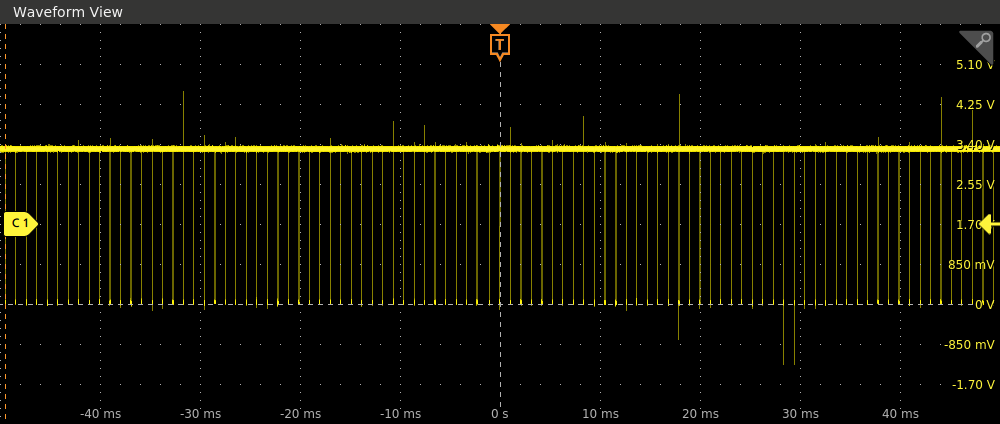
\includegraphics[scale=0.5]{assets/external-framework-value-wave.png}
  \caption{\label{fig:external-framework-value-wave}Voltage measurement of the GPIO used by the external benchmarking framework}
\end{figure}


\begin{table}[!ht]
  \centering
  \begin{tabular}{llll}
                        & \multicolumn{3}{c}{Time ($\mu$s)}                             \\ \cline{2-4} 
                        & \multicolumn{1}{c}{Mean} & Min  & \multicolumn{1}{c}{Max} \\ \cline{2-4} 
  Context switching time & 14.87                     & 14.79 & 14.97                    \\
  Duration of task 1    & 1003                     & 1003 & 1003                    \\
  Duration of task 2    & 1003                     & 1003 & 1003                   
  \end{tabular}
  \caption{Context switching times and task durations measured with the oscilloscope Tektronix MSO 56 using our external benchmarking framework}
  \label{tab:external-oscilloscope-framework-measurement}
\end{table}

\subsection{Discussion}